\section[Анализ предметной области]{АНАЛИЗ ПРЕДМЕТНОЙ ОБЛАСТИ}

\subsection{История развития велосипеда}

Велосипедист сегодняшних дней не может даже представить насколько запутанной
и удивительно интересной является история создания велосипеда.
На всём протяжении создания этого транспорта и его последующей трансформации
до современных форм происходило множество курьезов, фальсификаций и даже легендарных случаев.

Кого только не приписывали к авторам велосипедов. Французы твердо уверены,
что это техническое чудо изобрел их соотечественник граф де Сиврак еще в 1791 году.
Однако сам граф оказался выдумкой журналиста Луи Бодри, решившего в 1891 году
привить этому популярному транспортному средству французские корни.
Итальянцы дают отсылки на работы великого Леонардо и его ученика
Джакомо Капротти и предъявляют мировому сообществу сомнительные рисунки,
на которых изображен велосипед с цепной передачей. Наши соотечественники считают,
что изобретателем велосипеда был крестьянин Артамонов, который продемонстрировал
свою чудо-машину на коронации государя Павла Петровича в 1801 году.
Однако коронация Павла І проводилась в 1796 году, а проведенный недавно анализ
металла <<велосипеда Артамонова>> показывает, что его изготовили в 80-х годах 19 века.

Если покончить с выдумками и легендами, то первым достоверным конструктором
велосипеда можно считать жителя Карлсруэ, барона \textit{Карла фон Дреза}, предложившего
в 1817 году \textit{<<машину для ходьбы>>} --- первый прообраз велосипеда. Этот <<самокат>> имел раму,
колеса и руль, но не имел тормозной системы и цепной передачи. Конструкция была
выполнена из дерева и получила от современников название \textit{<<дрезина>>}.
Сложный в климатическом плане 1816 год, оставивший Европу без лошадей,
позволил <<дрезине>> получить самое широкое распространение и уже в 1818 году
конструкцию на Карла фон Дреза был получен \textit{патент}. Особой популярностью
это транспортное средство стало пользоваться в Англии, где его называли <<денди-хорз>>.

Популярность конструкции <<дрезины>> привлекла к этому транспорту внимание шотландца
\textit{Киркпатрика Макмиллана}, оснастившего конструкцию фон Дреза седлом и педалями,
что позволило не отталкиваться от земли ногами, а вращать заднее колесо
при помощи педалей и системы шатунов. Дальше Макмиллана в совершенствовании <<дрезин>>
пошел француз Пьер Лалман, поставивший в 1862 году педели на переднее колесо.
Такой вариант компоновки сохраняют до сих пор некоторые детские велосипеды.
Революционная идея позволяла приводить колесо в движение посредством вращения педелей,
а не толчков, как у Макмиллана.

Дальнейшие события развиваются стремительными темпами. В 1864 в паре с \textit{Лалманом}
инженер \textit{Пьер Мишо} создает металлическую раму и название \textit{<<велосипед>>}
для нового транспорта. В 1866 году \textit{Лалман} получает \textit{патент} на изобретение велосипеда.
Через год Каупер изобретает велосипедное колесо, состоящее из обода спиц и втулки.
Именно в этом виде конструкция колеса дошла до современных велосипедов.
В 1878 году английский изобретатель \textit{Лоусон} применяет цепную передачу на заднее колесо.

Эти новшества позволяют отойти от схемы <<пенни-фартинг>>, при которой переднее
или заднее колесо было значительно больше другого в колесной паре и
\textit{Джон Кемп Старли} патентует знаменитый \textit{Rover} --- практически полный аналог
современного велосипеда. Еще через десять лет шотландец \textit{Данлоп} предлагает
использовать в конструкции велосипеда каучуковые шины.

Следующее десятилетие вносит в конструкцию велосипеда такой элемент как педальный тормоз
и механизм свободного хода, обеспечивающий неподвижность педалей при движении велосипеда.
Начало нового века дарит велосипеду первый механизм переключения передач. В это время
он существует в очень неудобном варианте и не приживается до 1903 года, когда патентуют
планетарный механизм переключения передач. Окончательно этот узел конструкции велосипеда
меняется к середине ХХ века, когда итальянский велогонщик \textit{Компаньоло}
патентует современный вариант механизма переключения скоростей.

Вторая половина ХХ века вносит в конструкцию велосипеда новые материалы ---
\textit{титан} и \textit{карбон}. В конце прошлого века появляется механизм
индексного переключения передач.

Велосипед не только менялся сам на протяжении с 1817 года по конец XX века,
он менял людей и их пристрастия. Именно велосипед ввел в моду женские брюки и стал
одним из толчков для развития движения феминисток. Именно велосипед вводит моду
на здоровый образ жизни во второй половине XX века, и становиться образцом
экологически безупречного транспорта в конце этого столетия~\cite{bicycle_history}.

На рисунке~\ref{fig:bicycle_evolution} представлен процесс эволюции велосипеда
с 1818 года по наши дни.

\begin{figure}[h]
  \centering
  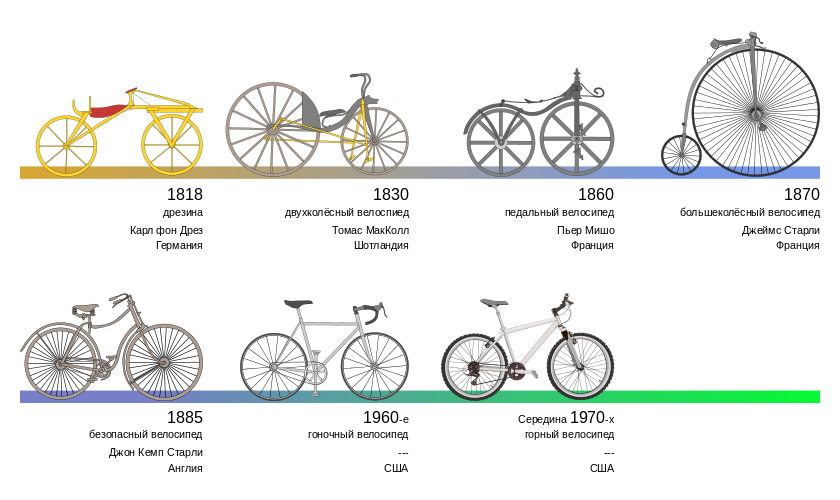
\includegraphics[width=150mm]{pic/bicycle_evolution.png}
  \caption{Эволюция велосипеда с 1818 года \\ по наши дни}
  \label{fig:bicycle_evolution}
\end{figure}


\subsection{История развития велосипедного спорта}

Первым крупным международным соревнованием была гонка на дистанции 120 км,
проходившая в \textit{1869 г.} во Франции по маршруту \textit{Париж-Руан},
участники которой выступали на деревянных велосипедах. В \textit{программу Олимпийских игр}
велоспорт был включен с 1896 года среди мужчин, а с 1984 года --- среди женщин.
На Олимпийских играх в период с 1896 года по 1924 год программа олимпийских
состязаний составлялась произвольно: в ряде случаев включались гонки только
на треке --- 1900 год и 1904 год, либо только на шоссе --- 1912 год.

\textit{Программа соревнований} стала определяться с 1928 года и мало изменялась до 1992 года.
Программа на треке предусматривала гит с места 1000 м --- именно здесь фиксируются рекорды,
а так же спринтерскую гонку, индивидуальную и командную гонки преследования 4000 м,
групповую и командную шоссейные гонки. В период с 1908 года по 1972 год
проводились трековые гонки на тандемах.

Каждая национальная команда могла быть представлена пятнадцатью гонщиками,
каждый заявленный спортсмен имел право
выступать в любой дисциплине. Однако регламент соревнований ограничивал
количество стартующих: в гите с места, спринтерской гонке и индивидуальной
гонке преследования на треке --- по одному спортсмену, в групповой шоссейной гонке --- по четыре,
в командной шоссейной гонке 100 км и командной гонке преследования на треке ---
по одной команде из четырех человек.

Командная и групповая шоссейные гонки проводятся раздельно с 1960 года.
До этого в командной гонке засчитывалась сумма результатов, показанных спортсменами
каждой из стран-участниц этих соревнований. В соревнованиях 1912 года учитывалась
сумма четырех, а в период с 1920 года по 1956 год --- сумма трех результатов.

В \textit{программу Олимпийских игр 1996 года} включены новые виды гонок для мужчин и женщин ---
индивидуальная гонка на шоссе и кросс, а исключена командная гонка на шоссе.
Таким образом, на Олимпийских играх разыгрывалось \textit{14 комплектов медалей:}
\begin{itemize}
  \item групповая шоссейная гонка у мужчин и женщин;
  \item индивидуальная гонка на время у мужчин и женщин;
  \item на треке --- гит 1000 м с места у мужчин;
  \item спринтерская гонка у мужчин и женщин;
  \item индивидуальная гонка преследования у мужчин и женщин;
  \item командная гонка преследования у мужчин;
  \item гонка по очкам у мужчин и женщин;
  \item маунтенбайк --- кросс-кантри у мужчин и женщин.
\end{itemize}

\textit{Чемпионаты мира по гонкам на треке} проводятся с 1893 года.
\textit{Чемпионаты мира по гонкам на шоссе} проводятся начиная с 1921 года,
а в закрытых помещениях с 1929 года.
Первый чемпионат мира по велосипедному спорту на треке состоялся в 1893 году в Чикаго,
США, а на шоссе --- в 1921 году в Копенгагене, Дания.

\textit{Чемпионаты мира по велокроссу} проводятся с 1950 года.
\textit{Чемпионаты Европы} проводятся только по гонкам в закрытых помещениях
начиная с 1930 года.
\textit{Международный союз велосипедистов UCI} был основан в 1900 году.
По состоянию на 1999 год в него входило 167 стран. В его состав, до 1992, входила
\textit{Международная любительская федерация велосипедного спорта --- ФИАК},
которая была основана в 1965 году, а также \textit{Международная федерация
профессионального велосипедного спорта --- ФИКП}.

Начиная с 1993 года разделение на любительскую и профессиональную федерации
признано нецелесообразным, и в настоящее время образован единый Международный
союз велосипедистов~\cite{bicycle_sport_history}.

\subsection{Велосипедное движение в Республике Беларусь}

\subsection{Актуальность разработки интернет-магазина \\ велосипедов}

\pagebreak
